\section{Deciphering Spanish Gigaword}
\label{decipher_spanish}
In this section, we describe data and experiment details for deciphering Spanish into English.

\subsection{Data}

In our Spanish-English decipherment experiments, we use half of the Gigaword corpus as monolingual data, and a small amount of parallel data from Europarl for evaluation. We keep only the top 10k most frequent word types for both languages and replace all other word types with ``UNK''.  We also exclude sentences with more than 40 tokens as longer sentences significantly slow down the parser we use. After preprocessing, the size of data for each language is shown in Table \ref{es-en-data}. The Gigaword corpus consists of news articles from different news agencies.  While we use all the monolingual data shown in Table \ref{es-en-data} to learn word embeddings, we only parse the AFP (Agence France-Presse) section of the corpus to extract cipher dependency bigrams and build a plaintext language model. We also use GIZA\cite{GIZA} to align a small amount of parallel data to build a dictionary for decipherment evaluation.

 \begin{table}
 \begin{center}
 \begin{tabular}{ |c|c|c| } \hline
             & Spanish & English \\ \hline
Non Parallel & \multirow{2}{*}{992 million} & \multirow{2}{*}{940 million} \\ 
(Gigaword) & &  \\ \hline
Parallel & \multirow{2}{*}{1.1 million} & \multirow{2}{*}{1.0 million} \\
(Europarl) & &  \\ \hline
 \end{tabular}
 \caption{Size of data in tokens used in Spanish-English decipherment}
 \label{es-en-data}
 \end{center}
 \end{table}

\subsection{Systems}
We implement a baseline system based on the work described in \newcite{dou-knight:2013:EMNLP}. The baseline system carries out decipherment on dependency bigrams.Therefore, we use Bohnet parser \cite{bohnet:2010:PAPERS} to parse AFP section of both Spanish and English version of Gigaword corpus. Since not all dependency relations are shared across the two languages, we do not extract all dependency bigrams. Instead, we only use bigrams with dependency relations in the following list: 

\begin{itemize}
\item Verb-Subject
\item Verb-Noun Object
\item Preposition-Preposition Object
\item Noun-Noun Modifier
\end{itemize}

The baseline uses slice sampling with uniform base distribution during decipherment.

We denote the system that uses our new method as \textbf{DMRE} (Dirichlet Multinomial Regression). The system is the same as the baseline except that it uses a base distribution derived from word context similarities.  The word embeddings are learned using word2vec \cite{mikolov2013efficient};

For all the systems, language models are built using the SRILM toolkit \cite{srilm}. We use modified Kneyser-Ney \cite{KneserNey95} algorithm for smoothing.


\subsection{Sampling Procedure}
\label{sample_procedure}

 \begin{figure}[!ht]
  \centering
  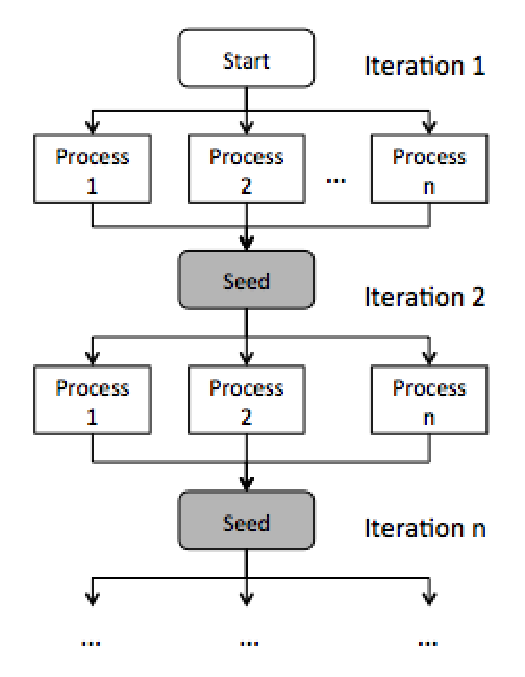
\includegraphics[width=2.9in,height=3.9in]{iterative_sampling}
  \caption{Iterative sampling procedures}
\label{iterative_sampling}
\end{figure}

Motivated by the previous work, we use multiple random restarts and iterative sampling process to improve decipherment \cite{Dou:2012}. As shown in Figure. The idea is to start a few sampling processes each with a different random sample. Then combine the results from different runs and use the combined results to initiate the next sampling iteration. The details of the sampling procedure are listed below:

 \begin{itemize}
  \item Extract dependency bigrams from parsing outputs and collect their counts.
  \item Keep bigrams whose counts are greater than a threshold $t$. Then start N different randomly seeded and initialized sampling processes. Perform sampling.
  \item At the end of sampling, extract word translation pairs $(f,e)$ from the final sample. Estimate translation probabilities $P(e|f)$  for each pair. Then construct a translation table by keeping translation pairs $(f,e)$ seen in more than one decipherment and use the average $P(e|f)$ as the new translation probability.
  \item Lower the threshold $t$ to include more bigrams into the sampling process. Start N different sampling processes again and initialize the first sample using the translation pairs obtained from the previous step (for each dependency bigram $f_{1},f_{2}$, find an English sequence $e_{1},e_{2}$, whose $P(e_{1}|f_{1})\cdot P(e_{2}|f_{2})\cdot P(e_{1},e_{2})$is the highest). Perform sampling again.
  \item Repeat until $t=1$.
\end{itemize}

In our Spanish-English decipherment experiments, we use 10 different random starts. In experiments, we also gradually increase the weight of base distribution as more and more ciphtertext becomes available. We set the weight to 2, 10, and 50 for ciphertext with 100k, 1 million, and 10 million tokens respectively. 

\subsection{Evaluation Metrics}
We use type accuracy as our evaluation metric: Given a word type $f$ in Spanish, we find top 5 translation pairs $(f,e)$ ranked by $P(e|f)$ from the translation table learned through decipherment. If the translation pair $(f,e)$ can also be found in a gold translation lexicon $T_{gold}$, we treat the word type $f$ as correctly deciphered. Let $|C|$ be the number of word types correctly deciphered, and $|V|$ be the total number of word types evaluated. We define type accuracy as $\frac{|C|}{|V|}$.

To create $T_{gold}$, we use GIZA to align a small amount of Spanish-English parallel text (1 million tokens for each language), and use the lexicon derived from the alignment as our gold translation lexicon. $T_{gold}$ contains a subset of 4233 word types in the top 5000 frequent word types, and 7479 word types in the top 10k frequent word types. We decipher top 10k frequent Spanish word types to top 10k frequent English word types, and evaluate decipherment accuracy on both top 5k most frequent word types and all the 10k word types.

\section{Deciphering Malagasy}
\label{decipher_malagasy}
In this section, we first introduce the Malagasy language, and describe the data used in the experiments; then explain what makes deciphering Malagasy more challenging compared with Spanish, and differences in experiment settings for achieving higher decipherment accuracy.

\subsection{The Malagasy Language}
Malagasy is the official language of Madagascar. It has around 18 million native speakers. Although Madagascar is an African country, Malagasy belongs to the Malayo-Polynesian branch of the Austronesian language family. Malagasy and English have very different word orders. First of all, in contrast to English, which has a subject-verb-object (SVO) word order, Malagasy has a verb-object-subject (VOS) word order. Besides that, Malagasy is a typical head initial language: Determiners precede nouns, while other modifiers and relative clauses follow nouns (e.g. ny ``the'' boky ``book'' mena ``red''). The significant differences in word order pose great challenges for decipherment.


\subsection{Data}
We list the size of both monolingual and parallel data used in this experiment in Table \ref{mlg-en-data}. The data used in this experiment is released from previous work by \newcite{dou-vaswani-knight:2014:EMNLP2014}. The monolingual data in Malagasy contains news data collected from various local websites. The English monolingual data contains Gigaword and additional 300 million tokens of news on Africa. The parallel data is collected from GlobalVoices, a multilingual news website, where volunteers translate news into different languages. The parallel data is used to build a dictionary for evaluating decipherment accuracy. 

 \begin{table}
 \begin{center}
 \begin{tabular}{ |c|c|c| } \hline
             & Malagasy & English \\ \hline
\multirow{2}{*}{Non Parallel} & 16 million & 1.2 billion\\ 
& (Web) & \pbox{2cm}{ (Gigaword \\ and Web)}  \\ \hline
\multirow{2}{*}{Parallel} & 2.0 million& 1.8 million \\
 & (GlobalVoices) & (GlobalVoices)  \\ \hline
 \end{tabular}
 \caption{Size of data in tokens used in Malagasy-English decipherment}
 \label{mlg-en-data}
 \end{center}
 \end{table}
 
\subsection{Systems}
The baseline system is the same as the baseline used in Spanish-English decipherment experiments. We use data provided in previous work \cite{dou-vaswani-knight:2014:EMNLP2014} to build a Malagasy dependency parser. For English, we use Turbo parser trained on Penn Treebank \cite{TurboParser}.  

Since the Malagasy parser doesn't predict dependency relation types, we use head-child part-of-speech (POS) tag patterns to select a subset of dependency bigrams for decipherment. We list the selected POS tag patterns in Table \ref{mlg-en-dep-type}.

%
 \begin{table}
 \begin{center}
 \begin{tabular}{ |c|c| } \hline
          Head POS & Child POS \\ \hline
Verb & Noun \\ \hline
Verb & Proper Noun \\ \hline
Verb & Person Pronoun \\ \hline
Preposition & Noun \\ \hline
Preposition & Proper Noun \\ \hline
Noun & Adjective \\ \hline
Noun & Determiner \\ \hline
Noun & Verb Particle \\ \hline
Noun & Verb Noun \\ \hline
Noun & Cardinal Number \\ \hline
Noun & Noun \\ \hline
 \end{tabular}
 \caption{Head-Child POS patterns used in decipherment}
 \label{mlg-en-dep-type}
 \end{center}
 \end{table}
%

\subsection{Sampling Procedure}
We use the same sampling protocol designed for Spanish-English decipherment. However, in experiments, we find out that simply using viterbi decoding to initialize the first sample does not work as well as in deciphering Spanish. Therefore, in addition to using Viterbi decoding, we also initialize the base distribution to the base distribution of previous decipherment that produces highest decipherment accuracy.

Compared with Spanish-English decipherment, we find the base distribution plays a more important role in achieving higher decipherment accuracy for Malagasy-English. Therefore, we set weight to 10, 100, and 500 when deciphering 100k, 1 million, and 20 million ciphtertext respectively.


%
 \begin{table*}[!ht]
 \begin{center}
 \begin{tabular}{ |c|c|c|c|c|c|c|c|c| } \hline
         & \multicolumn{4}{|c|}{Spanish-English} & \multicolumn{4}{|c|}{Malagasy-English} \\ \hline
 Top &  \multicolumn{2}{|c|}{5k} & \multicolumn{2}{|c|}{10k} & \multicolumn{2}{|c|}{5k} & \multicolumn{2}{|c|}{10k} \\ \hline
 System &  Baseline & DMRE & Baseline & DMRE &  Baseline & DMRE & Baseline & DMRE \\ \hline
 100k &  1.9 & 12.4 & 1.1 & 7.1 &  1.2 & 2.7 & 0.6 & 1.4 \\ \hline
 1 million &  7.3 & 37.7& 4.2 & 23.6 &  2.5 & 5.8 & 1.3 & 3.2 \\ \hline
 10 million &  26.0 & 59.1 & 15.9 & 43.7 &  5.4 & 11.2 & 3.0 & 6.9 \\ \hline
 \end{tabular}
 \caption{Spanish-English and Malagasy-English decipherment accuracy (\%) of top 5k and 10k most frequent word types}
 \label{decipher-acc-result}
 \end{center}
 \end{table*}
%

\subsection{Results}
In experiments, we gradually increase the size of ciphertext and compare decipherment accuracy of baseline with our new approach. We evaluate accuracy for top 5k and 10k most frequent word types for each language pair, and present them in Table \ref{decipher-acc-result}; 


 \begin{figure}[!ht]
  \centering
  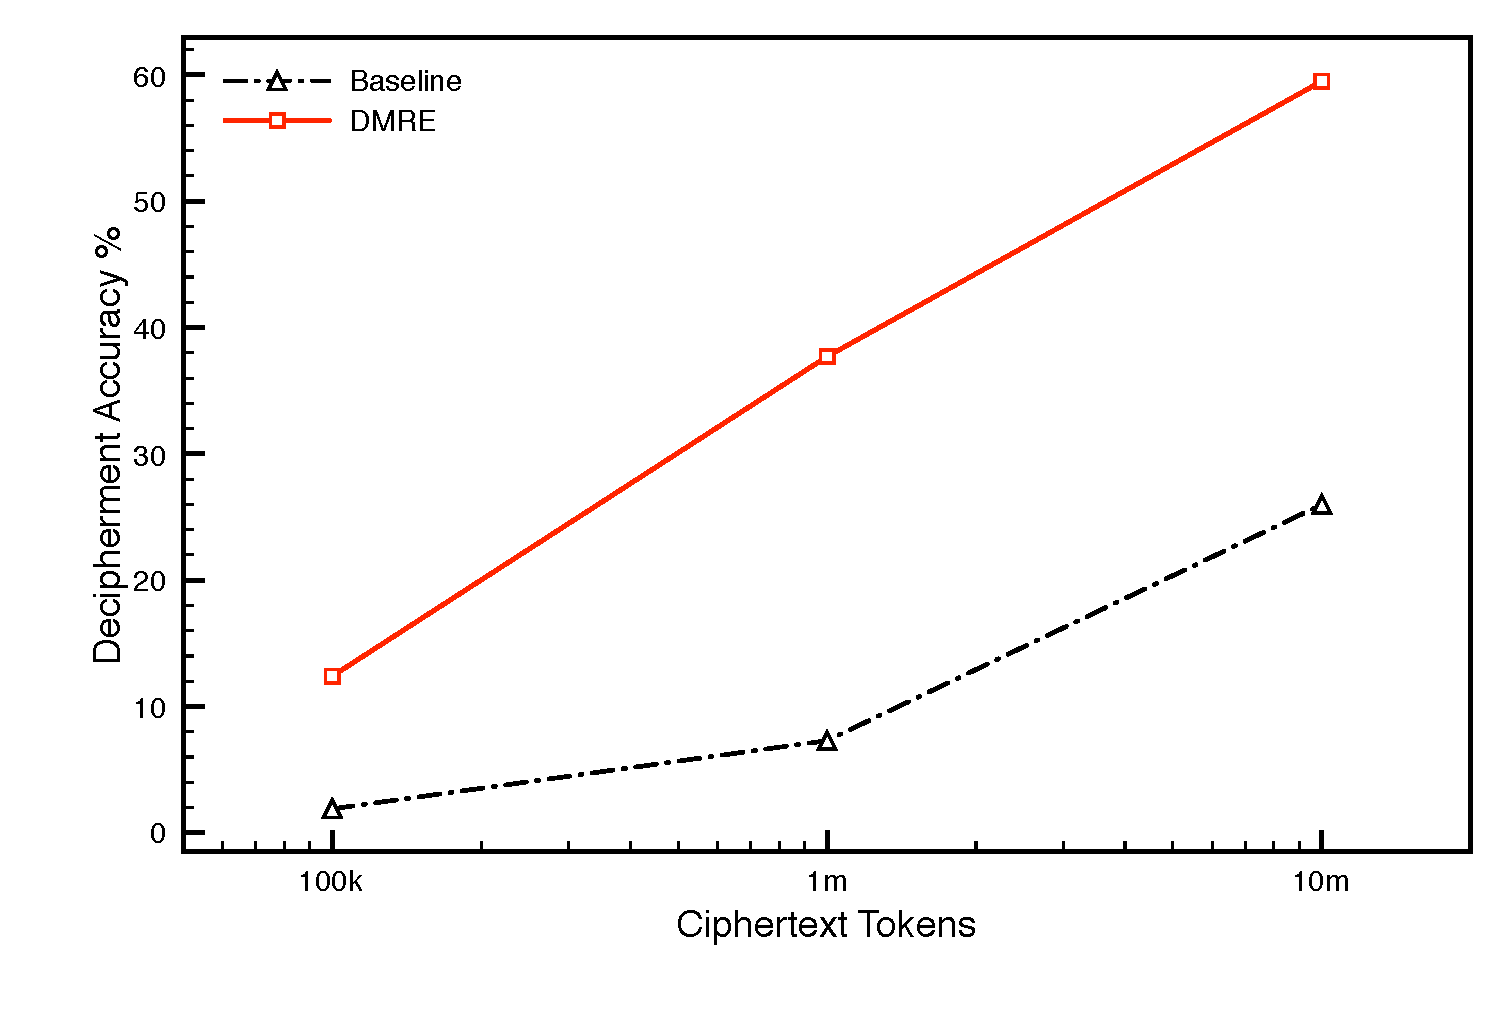
\includegraphics[width=3.1in,height=2.4in]{es_en_curve}
  \caption{Learning curves for Spanish-English decipherment.}
\label{es-en-curve}
\end{figure}

To better visualize the improvement, we also present the learning curves of decipherment accuracy for top 5k most frequent word types. Figure \ref{es-en-curve} compares baseline with \textbf{DMRE} in deciphering Spanish into English. Performance of the baseline is inline with previous work \cite{dou-knight:2013:EMNLP}. The accuracy reported here is higher as we evaluate top 5 accuracy for each word type. With 100k tokens of Spanish text, the baseline achieves 1.9\% accuracy, while the new system achieves 12.4\% accuracy, which improves the baseline by over 6 times. The improvement holds consistently throughout the experiment. In the end, the baseline achieves 26.0\% accuracy, while the new system achieves 59.1\% accuracy, over 2 times higher. 

 \begin{figure}[!ht]
  \centering
  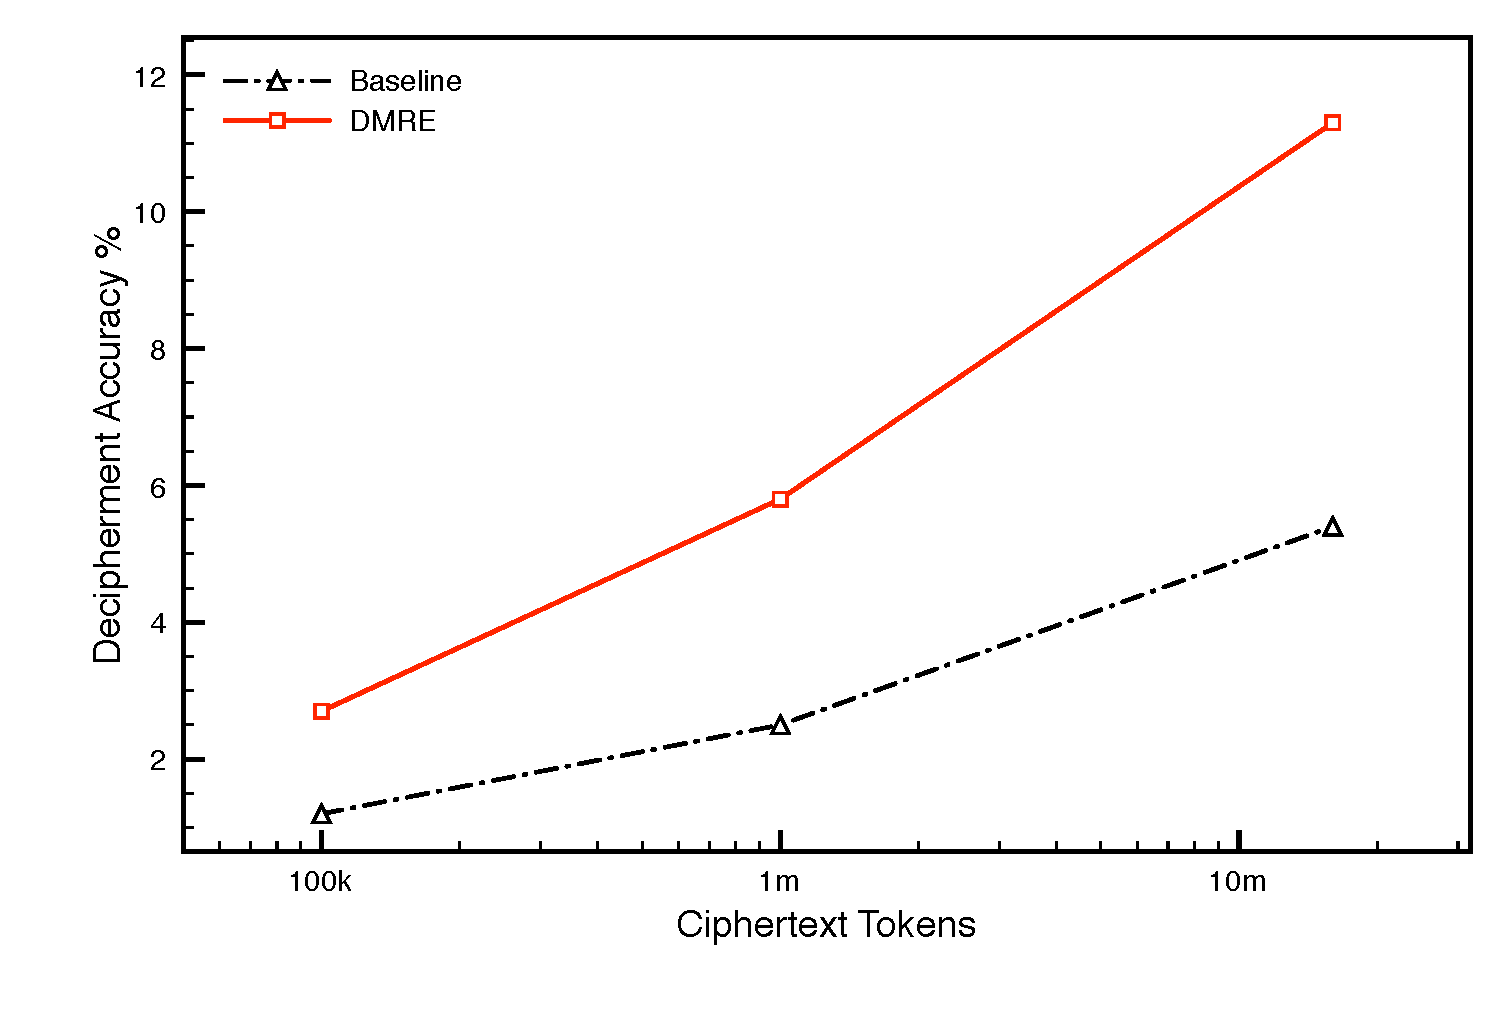
\includegraphics[width=3.1in,height=2.4in]{mlg_en_curve}
  \caption{Learning curves for Malagasy-English decipherment.}
\label{mlg-en-curve}
\end{figure}


Figure \ref{mlg-en-curve} compares baseline with our new approach in deciphering Malagasy into English. With 100k tokens of data, the baseline achieves 1.2\% accuracy, while the new system achieves 2.4\% accuracy.  We observe consistent improvement throughout the experiment. In the end, the baseline accuracy climbs to 5.8\%, while the new system improves it to 11.2\%.

Overall, the improvement we achieved is solid, and is observed across different language pairs. When we exam the base distribution, we find that the correct translations have higher probability. This helps prevent the language model driving deicpherment to a wrong direction. 

 





